\documentclass[preview]{standalone}

\usepackage[font=small]{caption}
\usepackage[labelformat=empty, position=top]{subcaption}
\usepackage{graphicx}
\usepackage[export]{adjustbox}
\usepackage{pgfplots}
\pgfplotsset{compat=newest}
\usepackage{amsmath,amsfonts,amssymb,bm}
\usepackage{mathptmx}%{times}
\usepackage{newtxtext}
\usepackage{newtxmath}
\usepackage{scalefnt}

\begin{document}

\begin{figure}

%%%%%%%%%%%%%%%%%%%%%%%%%%%%%%%%%%%%%%%%%%%%%%%%%%%%%%%%%%%%%%%%%%%%%%%%%%%%%%%%%%%%
% TEX
%%%%%%%%%%%%%%%%%%%%%%%%%%%%%%%%%%%%%%%%%%%%%%%%%%%%%%%%%%%%%%%%%%%%%%%%%%%%%%%%%%%%

  \begin{subfigure}[t]{0.05\textwidth}
    \vskip 0pt
    \textbf{\normalsize{(a)}}
  \end{subfigure}
  \hspace{0.02\textwidth}
  \begin{subfigure}[t]{0.39\textwidth}
    \vskip 0pt
    \resizebox{\textwidth}{!}{
      {\scalefont{1.25}
        \input{/project2/tas1/miyawaki/projects/002/figures/hahn/Control1850/native/dmse/mse_old/lo/0_poleward_of_lat_80/0_mon_r1_asym.tuned.tex}
      }
    }
  \end{subfigure}
  \hspace{0.02\textwidth}
  \begin{subfigure}[t]{0.05\textwidth}
    \vskip 0pt
    \textbf{\normalsize{(b)}}
  \end{subfigure}
  \hspace{0.02\textwidth}
  \begin{subfigure}[t]{0.39\textwidth}
    \vskip 0pt
    \resizebox{\textwidth}{!}{
      {\scalefont{1.25}
        \input{/project2/tas1/miyawaki/projects/002/figures/hahn/Flat1850/native/dmse/mse_old/lo/0_poleward_of_lat_80/0_mon_r1_asym.tuned.tex}
      }
    }
  \end{subfigure}

  \begin{subfigure}[t]{0.05\textwidth}
    \vskip 0pt
    \textbf{\normalsize{(c)}}
  \end{subfigure}
  \hspace{0.02\textwidth}
  \begin{subfigure}[t]{0.39\textwidth}
    \vskip 0pt
    \resizebox{\textwidth}{!}{
      {\scalefont{1.25}
        \input{/project2/tas1/miyawaki/projects/002/figures/hahn/Control1850/native/dmse/mse_old/lo/0_poleward_of_lat_80/0_mon_lh_asym.tuned.tex}
      }
    }
  \end{subfigure}
  \hspace{0.02\textwidth}
  \begin{subfigure}[t]{0.05\textwidth}
    \vskip 0pt
    \textbf{\normalsize{(d)}}
  \end{subfigure}
  \hspace{0.02\textwidth}
  \begin{subfigure}[t]{0.39\textwidth}
    \vskip 0pt
    \resizebox{\textwidth}{!}{
      {\scalefont{1.25}
        \input{/project2/tas1/miyawaki/projects/002/figures/hahn/Flat1850/native/dmse/mse_old/lo/0_poleward_of_lat_80/0_mon_lh_asym.tuned.tex}
      }
    }
  \end{subfigure}

  \begin{subfigure}[t]{0.18\textwidth}
    \hfill
  \end{subfigure}
  \begin{subfigure}[t]{0.7\textwidth}
    \vskip 0pt
    \resizebox{\textwidth}{!}{
      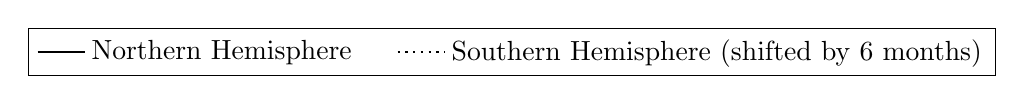
\begin{tikzpicture}
    \begin{axis}[
        hide axis,
        xmin=10,
        xmax=50,
        ymin=0,
        ymax=0.4,
        legend style={
            legend cell align=left,
            /tikz/every even column/.append style={column sep=0.5cm}
        },
        legend columns=-1,
    ]
    \addlegendimage{black, thick}
    \addlegendentry{Northern Hemisphere};
    \addlegendimage{black, thick, dotted}
    \addlegendentry{Southern Hemisphere (shifted by 6 months)};
    \end{axis}
\end{tikzpicture}

    }
  \end{subfigure}

%%%%%%%%%%%%%%%%%%%%%%%%%%%%%%%%%%%%%%%%%%%%%%%%%%%%%%%%%%%%%%%%%%%%%%%%%%%%%%%%%%%%
% PNG
%%%%%%%%%%%%%%%%%%%%%%%%%%%%%%%%%%%%%%%%%%%%%%%%%%%%%%%%%%%%%%%%%%%%%%%%%%%%%%%%%%%%

  % \begin{subfigure}[t]{0.05\textwidth}
  %   \textbf{\small{(a)}}
  % \end{subfigure}
  % \begin{subfigure}[t]{0.45\textwidth}
  %   \includegraphics[width=\textwidth, valign=t]{/project2/tas1/miyawaki/projects/002/figures/hahn/Control1850/native/dmse/mse_old/lo/0_poleward_of_lat_80/0_mon_r1_asym.png}
  % \end{subfigure}
  % \begin{subfigure}[t]{0.05\textwidth}
  %   \textbf{\small{(b)}}
  % \end{subfigure}
  % \begin{subfigure}[t]{0.45\textwidth}
  %   \includegraphics[width=\textwidth, valign=t]{/project2/tas1/miyawaki/projects/002/figures/hahn/Flat1850/native/dmse/mse_old/lo/0_poleward_of_lat_80/0_mon_r1_asym.png}
  % \end{subfigure}

  % \begin{subfigure}[t]{0.05\textwidth}
  %   \textbf{\small{(c)}}
  % \end{subfigure}
  % \begin{subfigure}[t]{0.45\textwidth}
  %   \includegraphics[width=\textwidth, valign=t]{/project2/tas1/miyawaki/projects/002/figures/hahn/Control1850/native/dmse/mse_old/lo/0_poleward_of_lat_80/0_mon_lh_asym.png}
  % \end{subfigure}
  % \begin{subfigure}[t]{0.05\textwidth}
  %   \textbf{\small{(d)}}
  % \end{subfigure}
  % \begin{subfigure}[t]{0.45\textwidth}
  %   \includegraphics[width=\textwidth, valign=t]{/project2/tas1/miyawaki/projects/002/figures/hahn/Flat1850/native/dmse/mse_old/lo/0_poleward_of_lat_80/0_mon_lh_asym.png}
  % \end{subfigure}

  % \begin{subfigure}[t]{0.14\textwidth}
  %   \hfill
  % \end{subfigure}
  % \begin{subfigure}[t]{0.75\textwidth}
  %   \includegraphics[width=\textwidth, valign=t]{/project2/tas1/miyawaki/projects/002/figures/hahn/Flat1850/native/dmse/mse_old/lo/0_poleward_of_lat_80/0_asym_leg.png}
  % \end{subfigure}

\end{figure}

\end{document}

